\def \makegans{
    \section{Mô hình Generative Adversarial Networks}
    \subsection{Giới thiệu chung}
    Ngày nay, công nghệ phát triển kéo theo nhu cầu sử dụng những nội dung số như hình ảnh, âm thanh hay video càng ngày càng lớn. Bên cạnh đó, cách mạng công nghiệp 4.0 cũng mang đến một nhu cầu lớn về dữ liệu để sử dụng trong các mô hình deep learning\index{deep learning}. Do đó, ta cần đến những mô hình sinh dữ liệu (generative model\index{generative model}) có khả năng tạo ra những bộ dữ liệu hoàn toàn mới và rất giống với những bộ dữ liệu do con người tạo ra, từ đó, cải thiện chất lượng của các mô hình deep learning\index{deep learning}.\\
    Generative Adversarial Networks\index{generative adversarial networks} \cite{gan} (hay gọi tắt là GANs\index{GANs}) được giới thiệu lần đầu vào năm 2014 bởi Ian Goodfellow và các cộng sự là ý tưởng cực kỳ độc đáo và là một bước tiến lớn gần đây trong lĩnh vực machine learning\index{machine learning} nói chung và computer vision nói riêng. Yann LeCun, VP and Chief AI Scientist, Facebook, từng mô tả về GANs: “The most interesting idea in the last 10 years in Machine Learning”, có thể hiểu như sau:"Là ý tưởng thú vị nhất trong 10 năm trở lại đây của lĩnh vực Machine Learning". Mục tiêu của GANs\index{GANs} là sinh ra được bộ dữ liệu mới có cùng những thông số thống kê với bộ dữ liệu đầu vào. Bên cạnh các mô hình sinh dữ liệu khác như mô hình Markov ẩn\index{mô hình Markov ẩn} hay Boltzmann machine\index{Boltzmann machine}, mô hình GANs\index{GANs} đã đạt được những thành tựu đáng ghi nhận trong thời gian gần đây.

    \begin{figure}[H]
    \centering
    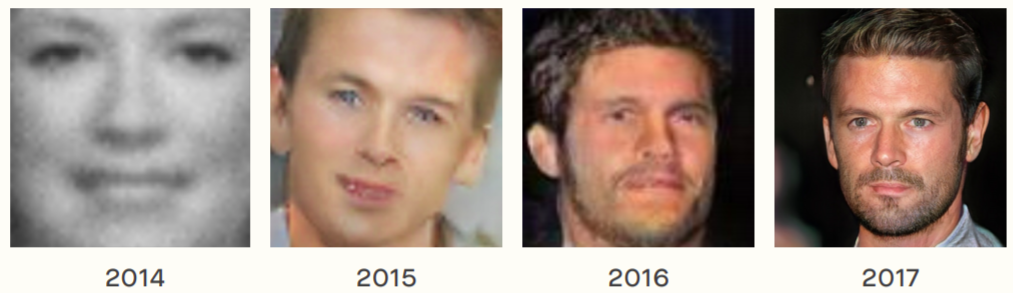
\includegraphics[width=12cm] {images/gan_results_timeline.png}
    \caption{Sự tiến bộ của mô hình GANs qua thời gian phát triển (Nguồn: \cite{malicious-gan})}
    \label{fig:gan_results_timeline}
    \end{figure}

    \noindent Thời điểm đầu, các mô hình GANs\index{GANs} chỉ có thể sinh ra những bức ảnh đơn giản như ảnh đen trắng hay ảnh có kích thước nhỏ. Tuy nhiên, cho đến nay, với sự phát triển của các mô hình GANs\index{GANs}, các mô hình như Progressive Growing GANs\index{Progressive Growing GANs} \cite{progressive-growing-gans}, StyleGAN\index{StyleGAN} \cite{style-gan}, StyleGAN2\index{StyleGAN2} \cite{style-gan2} đã mang đến những kết quả hết sức ấn tượng trong việc sinh ra ảnh có độ phân giải cao (lên tới 1024x1024 pixel). Đi cùng với đó, việc phân biệt được đâu là dữ liệu có thật và đâu là dữ liệu do mô hình GANs\index{GANs} sinh ra cũng đã trở thành một bài toán hóc búa. Deepfake Detection Challenge là một cuộc thi với giải thưởng rất lớn với bài toán phân biệt giữa ảnh thật và ảnh giả sinh ra bởi GANs\index{GANs}.
    
    \begin{figure}[H]
    \centering
    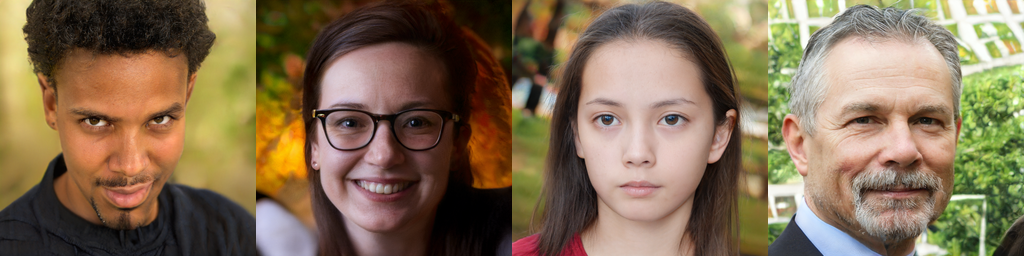
\includegraphics[width=12cm] {images/result_stylegan2.png}
    \caption{Kết quả rất xuất sắc mà mô hình GANs có thể sinh ra trong thời gian gần đây (Nguồn: \cite{style-gan2})}
    \label{fig:result_stylegan2}
    \end{figure}
    
    \noindent Các mô hình GANs\index{GANs} thường tập trung giải quyết các bài toán chính sau:
    \begin{itemize}[leftmargin=0cm,itemindent=.5cm,labelwidth=\itemindent,labelsep=0cm,align=left]
      \item \textbf{Image synthesis\index{Image synthesis}:} Sinh ra ảnh mới từ nhiễu. Một số mô hình nổi tiếng giải quyết bài toán này là Progressive Growing GANs\index{Progressive Growing GANs} \cite{progressive-growing-gans}, StyleGAN\index{StyleGAN} \cite{style-gan}, StyleGAN2\index{StyleGAN2} \cite{style-gan2} ...
      \item \textbf{Image-to-Image Translation\index{Image-to-Image Translation}:} Sinh ra ảnh mới từ ảnh đầu vào. Một số mô hình nổi tiếng giải quyết bài toán này là CycleGAN\index{CycleGAN} \cite{cycle-gan}, BicycleGAN\index{BicycleGAN} \cite{bicyle-gan}, MUNIT\index{MUNIT} \cite{munit} ...
      \item \textbf{Text-to-Image Translation\index{Text-to-Image Translation}:} Sinh ra ảnh mới từ một đoạn văn bản. Mô hình nổi tiếng giải quyết bài toán này là StackGAN\index{StackGAN} \cite{stack-gan} ...
      \item Ngoài các bài toán chính ở trên, mô hình GANs còn được sử dụng để sinh ra âm nhạc như trong bài báo \cite{midinet} ...
    \end{itemize}

    \subsection{Ý tưởng chính}
    Kiến trúc của GANs\index{GANs} bao gồm 2 phần: Generator\index{generator} và Discriminator\index{discriminator}. Một cách khái quát, Generator\index{generator} được luyện sao cho sinh ra được dữ liệu càng giống dữ liệu thật càng tốt. Bên cạnh đó, Discriminator\index{discriminator} được luyện sao cho có thể phân biệt được đâu là dữ liệu thật, đâu là dữ liệu giả được sinh ra bởi Generator\index{generator}.\\
    Ý tưởng của mô hình GANs\index{GANs} bắt nguồn từ zero-sum non-cooperative game, hiểu đơn giản như trò chơi đối kháng theo lượt gồm hai người, nếu một người thắng thì người còn lại sẽ thua. Ở mỗi lượt thi đấu, cả hai đối thủ đều muốn tối đa hoá cơ hội thắng của mình và tối thiểu hoá cơ hội thắng của đối phương. Discriminator\index{discriminator} và Generator\index{generator} trong mô hình GANs\index{GANs} giống như hai đối thủ trong trò chơi. Trong lý thuyết trò chơi thì mô hình GANs\index{GANs} đạt tới điểm hội tụ khi cả Generator\index{generator} và Discriminator\index{discriminator} đạt tới trạng thái cân bằng Nash\index{trạng thái cân bằng Nash}, tức là 2 người chơi đạt trạng thái cân bằng và đi tiếp các bước không làm tăng cơ hội thắng cho bất kỳ ai.

    \begin{figure}[H]
    \centering
    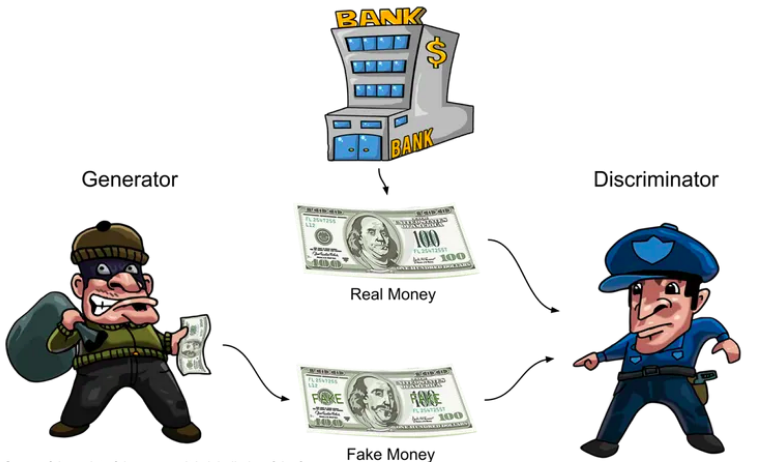
\includegraphics[width=12cm] {images/gans_example.png}
    \caption{Ví dụ mô phỏng mô hình GANs (Nguồn: dzone.com)}
    \label{fig:gans_example}
    \end{figure}
    
    \noindent Generator\index{generator} trong mô hình GANs giống như tên trộm làm tiền giả còn Discriminator\index{discriminator} giống như người cảnh sát. Tên trộm làm tiền giả sẽ cố gắng làm ra tiền giả mà người cảnh sát cũng không phân biệt được. Còn cảnh sát sẽ cố gắng phân biệt đâu là tiền thật được in bởi ngân hàng và đâu là tiền giả được làm ra bởi tên trộm. Mục tiêu cuối cùng là tên trộm làm tiền giả là làm ra tiền mà cảnh sát cũng không phân biệt được đâu là thật và đâu là giả và có thể sử dụng như tiền thật.\\
    Trong quá trình trên thì cảnh sát có nhiệm vụ là học cách phân biệt tiền nào là thật, tiền nào là giả và sau những lần tiền giả do tên trộm làm ra bị phát hiện thì tên trộm sẽ cần phải cải thiện hơn để tờ tiền giả trở nên tinh vi hơn. Dần dần, thì tên trộm làm tiền giả sẽ làm tiền giống tiền thật hơn và cảnh sát cũng thành thạo việc phân biệt tiền giả và tiền thật hơn. Và mục tiêu cuối cùng của quá trình huẩn luyện mô hình là tiền giả từ tên trộm làm tiền giả (đại diện cho Generator\index{generator}) sẽ đánh lừa được người cảnh sát (đại diện cho Discriminator\index{discriminator}).
    
    \begin{figure}[H]
    \centering
    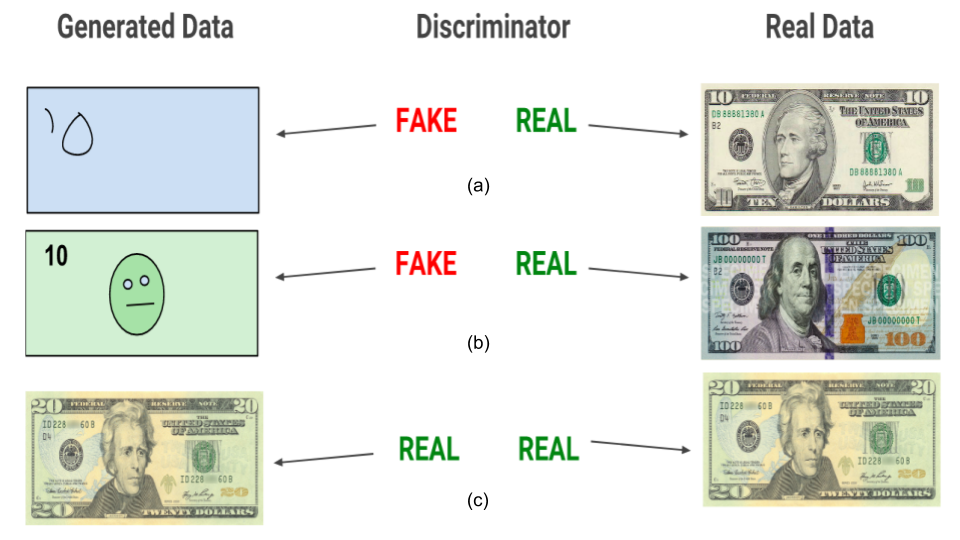
\includegraphics[width=12cm] {images/fake_vs_real.png}
    \caption{Kết quả của mô hình GANs (a) Giai đoạn đầu của quá trình luyện (b) Trong quá trình luyện (c) Sau khi được luyện hoàn chỉnh (Nguồn: tensorflow.org)}
    \label{fig:fake_vs_real}
    \end{figure}
    
    \noindent Trong giai đoạn đầu của quá trình huấn luyện, Generator\index{generator} sinh ra những bức ảnh rất đơn giản. Do đó, Discriminator\index{discriminator} dễ dàng phân biệt được ảnh thật và ảnh giả. Sau một khoảng thời gian, Generator bắt đầu sinh ra những bức ảnh phức tạp hơn, tuy nhiên, những kết quả này vẫn chưa đủ để đánh lừa được Discriminator\index{discriminator}. Cuối cùng, nếu Generator\index{generator} được luyện một cách hoàn chỉnh, nó có thể sinh ra những bức ảnh gần như giống và rất khó phân biệt với ảnh thật.
    
    \subsection{Chi tiết kiến trúc}
    \subsubsection{Kiến trúc của mô hình}
    \noindent Trong kiến trúc của mô hình GANs, Discriminator nhận đầu vào từ hai nguồn:

    \begin{itemize}[leftmargin=0cm,itemindent=.5cm,labelwidth=\itemindent,labelsep=0cm,align=left]
      \item Dữ liệu thật (VD: ảnh được chụp bởi con người) được dùng như là positive sample trong quá trình luyện.
      \item Dữ liệu giả (VD: ảnh được sinh ra bởi Generator) được dùng như là negative sample trong quá trình luyện.
    \end{itemize}
    
    \noindent và đầu ra của Discriminator\index{discriminator} được sử dụng trong discriminator loss\index{discriminator loss} và generator loss\index{generator loss}. Tuy nhiên, trong quá trình luyện Discriminator\index{discriminator}, nó chỉ sử dụng kết quả từ discriminator loss\index{discriminator loss} để cập nhật lại các trọng số. Discriminator\index{discriminator} sẽ bị phạt bởi discriminator loss\index{discriminator loss} nếu đưa ra dự đoán ảnh thật là giả hoặc ảnh giả là thật.\\
    Khác với Discriminator\index{discriminator}, Generator\index{generator} chỉ nhận một đầu vào ngẫu nhiên và biến đổi nó trở thành một điểm dữ liệu. Đầu ra của Generator\index{generator} được sử dụng làm đầu vào cho Discriminator\index{discriminator}, sau đó, điểm dữ liệu này được tính loss bởi generator loss\index{generator loss} và cập nhật lại các trọng số cho generator\index{generator}. Generator\index{generator} sẽ bị phạt nếu điểm dữ liệu nó tạo ra bị Discriminator\index{discriminator} dự đoán là giả.
    
    \begin{figure}[H]
    \centering
    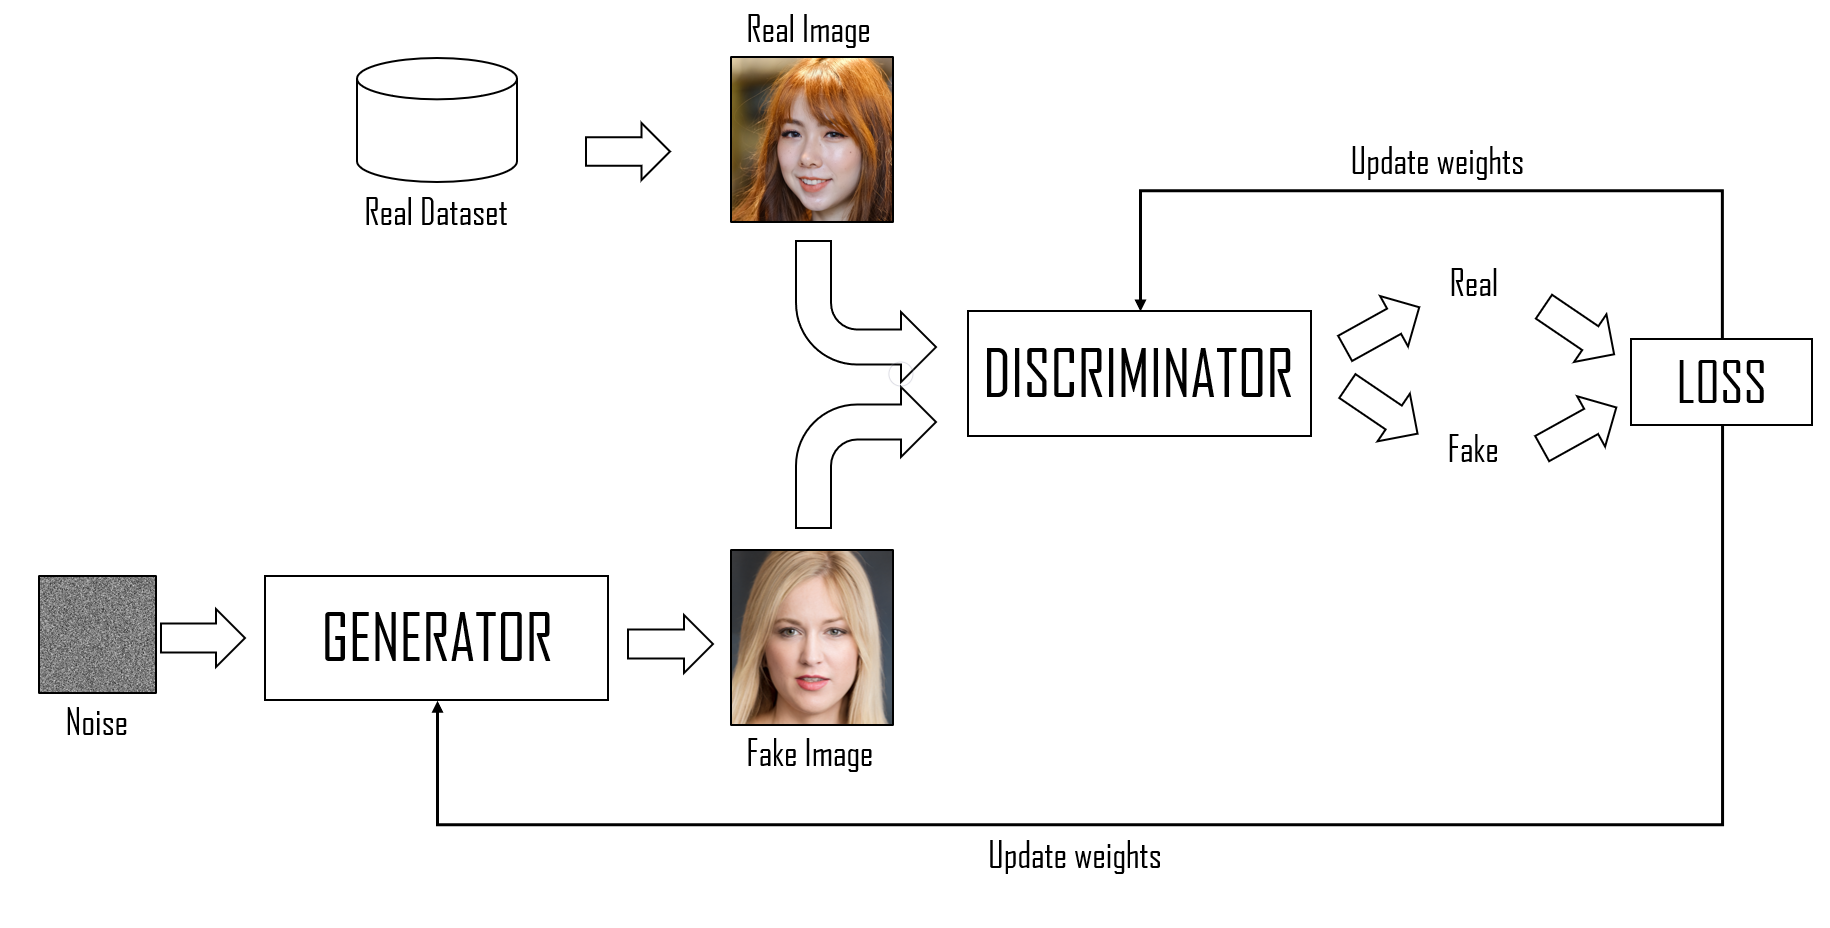
\includegraphics[width=13cm] {images/gans_model.png}
    \caption{Kiến trúc tổng quát của mô hình GANs}
    \label{fig:gans_model}
    \end{figure}
    
    \subsubsection{Hàm loss của mô hình}
    \noindent Một điểm rất đáng chú ý trong mô hình GANs là hàm loss. Hàm loss của GANs là Minimax loss\index{minimax loss}, trong khi Generator\index{generator} cố gắng tối thiểu hoá giá trị thì Discriminator\index{discriminator} được huấn luyện để tối đa hoá giá trị của nó. Vì Discriminator\index{discriminator} có nhiệm vụ phân biệt được đâu là ảnh thật, đâu là ảnh giả cho nên đây là bài toán phân lớp nhị phân\index{phân lớp nhị phân} (binary classification\index{binary classification}). Hàm loss lúc này của mô hình GANs\index{GANs} có dạng giống với hàm loss binary cross-entropy loss\index{loss binary cross-entropy loss}:
    \begin{align}
    \min_G \max_D V(D, G) = \mathbb{E}_{\bm{x} \sim p_{\text{data}}(\bm{x})}[\log D(\bm{x})] + \mathbb{E}_{\bm{z} \sim p_{\bm{z}}(\bm{z})}[\log (1 - D(G(\bm{z})))]
    \label{func:gan_loss}
    \end{align}
    trong đó:
    \begin{itemize}[leftmargin=0cm,itemindent=.5cm,labelwidth=\itemindent,labelsep=0cm,align=left]
        \item $x$ là điểm dữ liệu thật.
        \item $D(x)$ là xác suất mà Discriminator\index{discriminator} dự đoán $x$ là dữ liệu thật.
        \item $E_x$ là kỳ vọng đối với các giá trị của dữ liệu thật $x$.
        \item $z$ là đầu vào ngẫu nhiên của Generator\index{generator}.
        \item $G(z)$ là điểm dữ liệu được sinh ra bởi Generator\index{generator}.
        \item $D(G(z))$ là xác suất mà Discriminator\index{discriminator} dự đoán $G(z)$ là dữ liệu thật.
        \item $E_z$ là kỳ vọng đối với các giá trị ngẫu nhiên $z$.
    \end{itemize}
    Giá trị đầu ra của Discriminator\index{discriminator} được đưa qua layer sigmoid\index{sigmoid} nên có giá trị nằm trong khoảng [0, 1]. Do đó, Discriminator\index{discriminator} sẽ được huấn luyện để nếu đầu vào là ảnh từ bộ dữ liệu thì đầu ra gần 1, còn nếu đầu vào là ảnh sinh ra từ Generator\index{generator} thì đầu ra gần 0, hay nói cách khác $D(x)$ tiến dần đến 1 còn $D(G(z))$ tiền gần về 0. Từ đó, hàm loss của mô hình GANs\index{GANs} muốn cực đại hoá $D(x)$ và cực tiểu hoá $D(G(z))$. Việc cực tiểu hoá $D(G(z))$ tương đương với việc cực đại hoá $(1 - D(G(z))$. Vì vậy, ta có thể nói Discriminator\index{discriminator} được huấn luyện để cực đại hoá hàm loss của mô hình GANs\index{GANs}.
    \begin{align}
    \max_D V(D) = \mathbb{E}_{\bm{x} \sim p_{\text{data}}(\bm{x})}[\log D(\bm{x})] + \mathbb{E}_{\bm{z} \sim p_{\bm{z}}(\bm{z})}[\log (1 - D(G(\bm{z})))]
    \label{func:dis_loss}
    \end{align}
    Generator\index{generator} được huấn luyện để đánh lừa Discriminator\index{discriminator} rằng dữ liệu nó sinh ra là dữ liệu thật. Điều này đồng nghĩa với việc nó cố gắng để giá trị $D(G(z))$ càng tiến gần về 1 càng tốt hay nói cách khác là cực đại hoá $D(G(z))$. Việc cực đại hoá $D(G(z))$ tương đương với việc cực tiểu hoá $(1 - D(G(z))$. Bên cạnh đó, đối với Generator\index{generator} thì giá trị của $D(x)$ không phụ thuộc vào $G$ và luôn không đổi. Vì vậy, ta có thể nói Generator\index{generator} được huấn luyện để cực tiểu hoá hàm loss của mô hình GANs\index{GANs}.
    \begin{align}
    \min_G V(G) = \mathbb{E}_{\bm{z} \sim p_{\bm{z}}(\bm{z})}[\log (1 - D(G(\bm{z})))]
    \label{func:gen_loss}
    \end{align}
    Từ hàm loss của mô hình GANs\index{GANs}, ta có thể thấy là việc huấn luyện song song Generator\index{generator} và Discriminator\index{discriminator} là đối nghịch nhau, trong khi Discriminator\index{discriminator} cố gắng cực đại hoá giá trị hàm loss thì Generator\index{generator} cố gắng cực tiểu hoá giá trị hàm loss. Quá trình huấn luyện GANs\index{GANs} kết thúc khi mô hình GANs\index{GANs} đạt đến trạng thái cân bằng Nash của hai thành phần trong mô hình.
    
    \subsection{Phương pháp đánh giá}
    Bất kỳ mô hình deep learning\index{deep learning} nào cũng cần các phương pháp đánh giá xem mô hình đó hoạt động tốt ra sao, hay so sánh kết quả giữa các mô hình khác nhau. Việc đánh giá ảnh đầu ra theo quan điểm cá nhân của từng nguời không thật sự khách quan và khó áp dụng với lượng dữ liệu lớn mà các mô hình GANs\index{GANs} có thể sinh ra. Do đó, ta cần nghiên cứu các phương pháp để đánh giá chất lượng ảnh do các mô hình GANs\index{GANs} sinh ra chất lượng tốt hay không.\\
    Để đánh giá chất lượng của một mô hình GANs\index{GANs}, ta quan tâm tới hai yếu tố:
    \begin{itemize}[leftmargin=0cm,itemindent=.5cm,labelwidth=\itemindent,labelsep=0cm,align=left]
        \item Chất lượng ảnh: các ảnh sinh ra có giống với ảnh thật từ bộ dữ liệu có sẵn hay không?
        \item Độ đa dạng: các ảnh sinh ra có đa dạng hay không?
    \end{itemize}
    Dựa trên kết quả của mô hình phân loại ảnh InceptionNet\index{InceptionNet}, điểm inception\index{điểm inception} (Inception Score\index{inception score} gọi tắt là IS\index{IS}) được tính bằng cách sử dụng pretrained\index{pretrained} của mô hình InceptionNet\index{InceptionNet} trên bộ dữ liệu ImageNet\index{ImageNet}. Nếu một ảnh được đưa qua mô hình pretrained\index{pretrained} InceptionNet\index{InceptionNet}, giá trị đầu ra, do được đi qua lớp softmax\index{softmax}, nên sẽ là xác suất ảnh đầu vào đó thuộc từng lớp tương ứng. Việc dùng mô hình pretrained\index{pretrained} sẽ giúp kết quả đầu ra này tương đối đáng tin.\\
    Từ ý tưởng trên, ta có thể kiểm tra được chất lượng của ảnh đầu ra bằng việc đánh giá các giá trị xác suất tương ứng với mỗi lớp của InceptionNet\index{InceptionNet}. Nếu ảnh chất lượng cao, sau khi đi qua InceptionNet\index{InceptionNet} sẽ cho xác suất ảnh rơi vào một lớp cụ thể cao hơn hẳn các lớp khác. Ngược lại, nếu xác suất của các lớp đầu ra của InceptionNet\index{InceptionNet} tương đối cân bằng nhau (nghĩa là mô hình không nhận ra được đối tượng cụ thể trong ảnh), đồng nghĩa với việc chất lượng ảnh là không tốt. Trong hình \ref{fig:inception}, ảnh trên là kết quả của ảnh rõ nét mang lại kết quả chênh lệch giữa các lớp, ảnh dưới là kết quả của ảnh không rõ nét dẫn đến các kết quả cân bằng giữa các lớp.\\
    
    \begin{figure}[H]
    \centering
    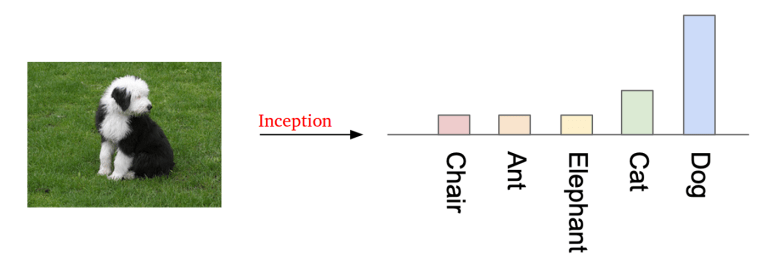
\includegraphics[width=10cm] {images/inception_1.png}
    \\[\smallskipamount]
    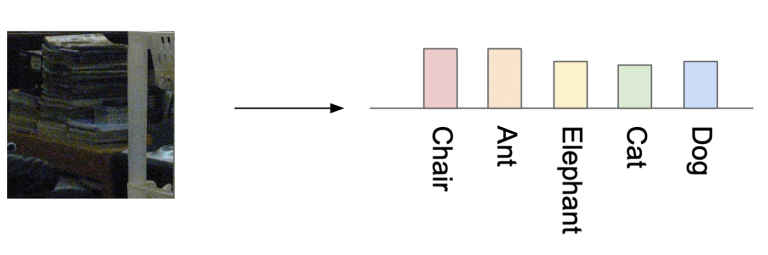
\includegraphics[width=9.5cm] {images/inception_2.png}
    \caption{Kết quả kiểm tra chất lượng của ảnh bằng cách đi qua mô hình pretrained\index{pretrained} InceptionNet\index{InceptionNet} (Nguồn: medium.com)}
    \label{fig:inception}
    \end{figure}
    
    \noindent Đối với độ đa dạng của ảnh, ta tính tổng các giá trị xác suất đầu ra theo từng lớp của các ảnh với mô hình pretrained\index{pretrained} InceptionNet\index{InceptionNet}. Nếu tổng này là các giá trị cân bằng giữa các lớp, thì ảnh đầu vào sinh ra bởi Generator\index{generator} có sự đa dạng giữa các lớp. Ngược lại, với bộ ảnh đầu ra thiếu đa dạng, thì tổng các giá trị xác suất theo lớp lúc này chỉ tập trung vào một vài lớp nhất định.
    
    \begin{figure}[H]
    \centering
    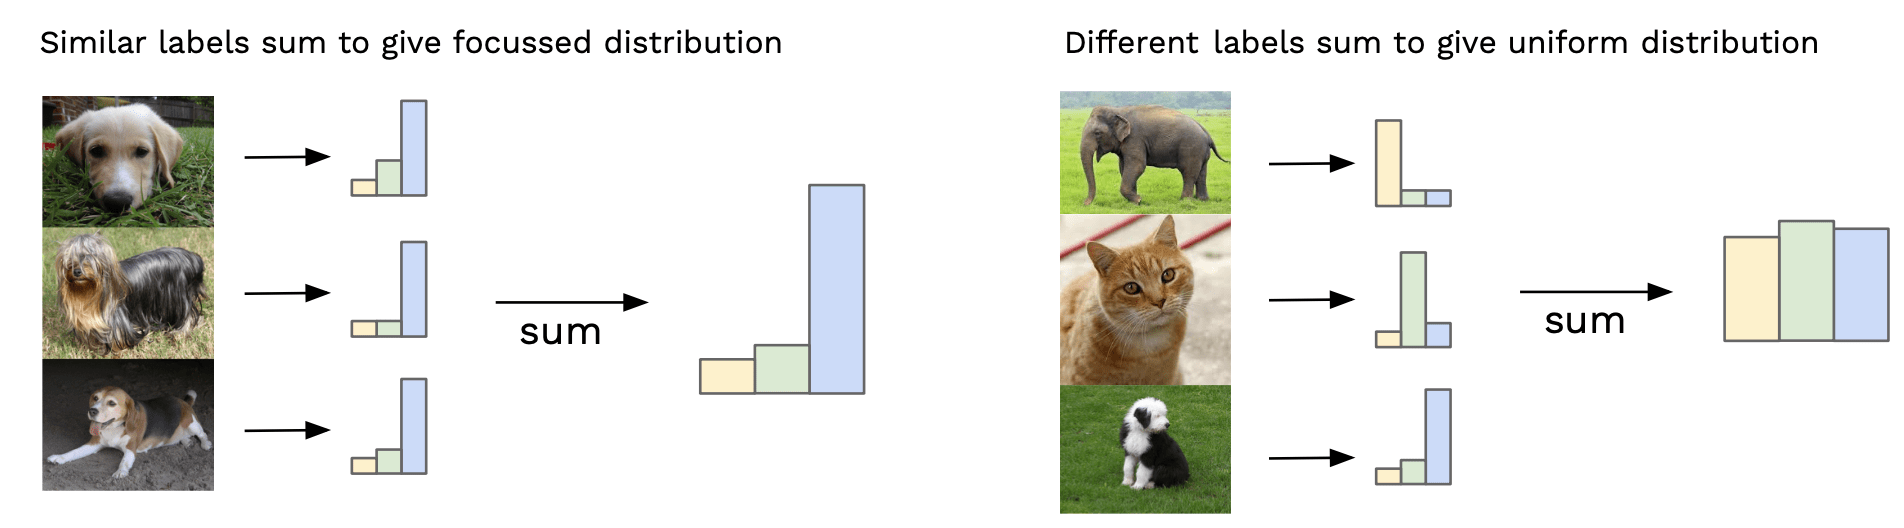
\includegraphics[width=13cm] {images/inception_3.png}
    \caption{Kết quả kiểm tra độ đa dạng của ảnh bằng cách đi qua mô hình pretrained\index{pretrained} InceptionNet\index{InceptionNet} (Nguồn: medium.com)}
    \label{fig:inception}
    \end{figure}
    \noindent Ta tính điểm inception\index{điểm inception} bằng công thức Kullback–Leibler divergence\index{Kullback–Leibler divergence} (gọi tắt là KL divergence\index{KL divergence}). KL divergence\index{KL divergence} nhận đầu vào là hai phân phối xác suất\index{phân phối xác suất} và đưa đầu ra là độ tương đồng giữa hai phân phối đó. Nếu 2 phân phối đó gần giống nhau thì giá trị KL divergence\index{KL divergence} gần tới 0, còn nếu hai phân phối càng khác nhau thì giá KL divergence\index{KL divergence}càng lớn.
    \begin{align}
        D_{KL}(P||Q) = \intP(x)\log\frac{P(x)}{Q(x)}dx
    \end{align}
    Ta gọi xác suất với đầu ra của InceptionNet\index{InceptionNet} là lớp $y$ với ảnh đầu vào $x$ là $P(y|x)$, giá trị này được gọi là label distribution\index{label distribution}. Ngoài ra, ta gọi tổng các label distribution\index{label distribution} của tất cả các ảnh đầu vào (đã được chuẩn hoá) là $P(y)$, giá trị này được gọi là marginal distribution\index{marginal distribution}. Quan hệ giữa hai phân phối xác suất này và giá trị KL divergence\index{KL divergence} được mô tả ở hình \ref{fig:is_kl}.\\
    Để ảnh sinh ra từ mô hình GANs\index{GANs} tốt (chất lượng ảnh tốt và đa dạng), thì ta muốn label distribution\index{label distribution} cao ở một lớp, thấp ở các lớp khác và marginal distribution\index{marginal distribution} cân bằng giữa các lớp, khi đó, hai phân phối xác suất này khác xa nhau, dẫn đến giá trị KL divergence\index{KL divergence} cao. Nếu label distribution\index{label distribution} cao ở nhiều lớp và marginal distribution\index{marginal distribution} cân bằng giữa các lớp thì giá trị KL divergence\index{KL divergence} cũng không cao. Nếu label distribution\index{label distribution} cân bằng và marginal distribution\index{marginal distribution} cũng có dạng cân bằng thì giá trị KL divergence\index{KL divergence} cũng thấp.\\
    \begin{figure}[H]
    \centering
    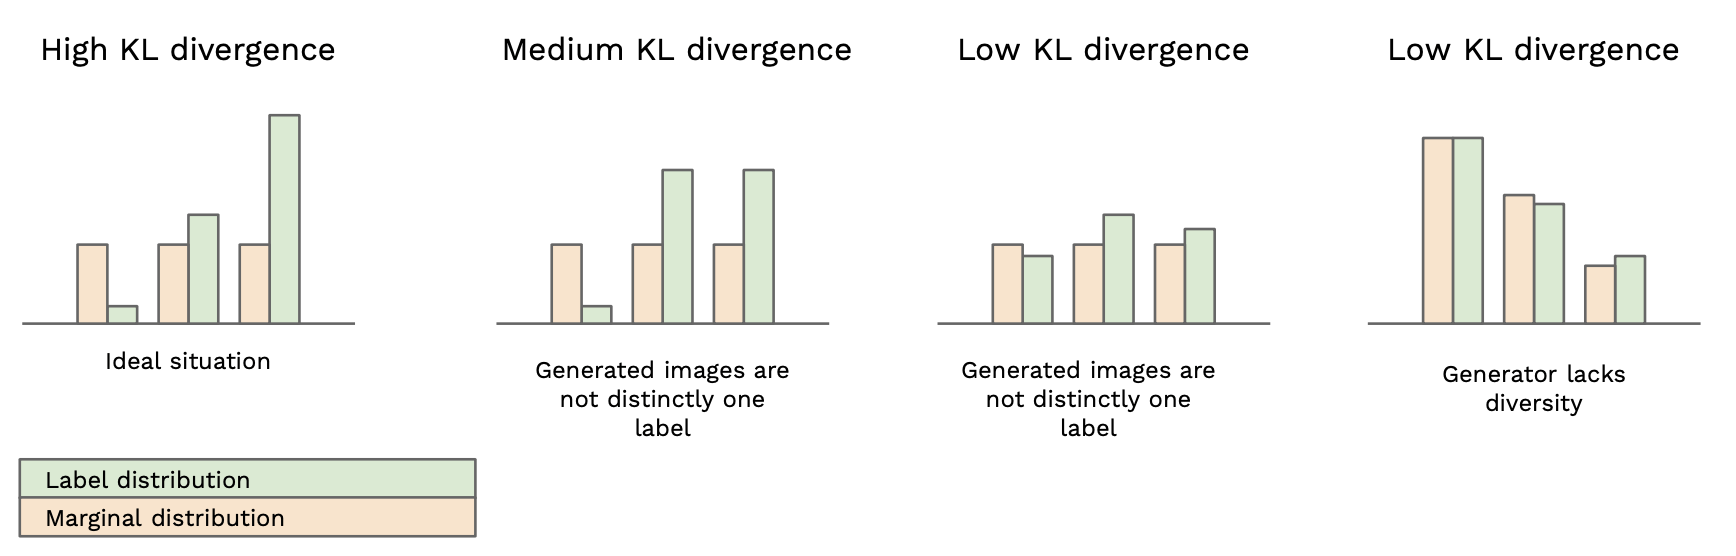
\includegraphics[width=13cm] {images/is_kl.png}
    \caption{Mối liên hệ giữa xác suất đầu ra của InceptionNet và KL divergence (Nguồn: medium.com)}
    \label{fig:is_kl}
    \end{figure}
    
    \noindent Giá trị KL divergence\index{KL divergence} sẽ cao khi ảnh chất lượng cao và ảnh đa dạng. Do đó, ta có thể tính giá trị KL divergence\index{KL divergence} cho mỗi ảnh sinh ra và tính trung bình các giá trị đó để tính điểm inception\index{điểm inception} cho mô hình GANs.
    \begin{align}
        IS(G) = \exp(\mathbb{E}_{\bm{x} \sim p_{\bm{g}}(\bm{x})}D_{KL}(p(y)||p(y|x)))
    \end{align}
    Điểm inception\index{điểm inception} được sử dụng rất nhiều trong việc đánh giá chất lương ảnh sinh ra từ một mô hình GANs\index{GANs}. Tuy nhiên, nó cũng có các hạn chế:

    \begin{itemize}[leftmargin=0cm,itemindent=.5cm,labelwidth=\itemindent,labelsep=0cm,align=left]
        \item Điểm inception\index{điểm inception} dựa vào mô hình InceptionNet\index{InceptionNet} được pretrained\index{pretrained} với bộ dữ liệu ImageNet\index{ImageNet}, do đó, với những ảnh sinh ra bởi mô hình GANs\index{GANs} nhưng không thuộc các lớp có sẵn trong bộ dữ liệu ImageNet\index{ImageNet} thì kết quả này cũng không đáng tin.
        \item Trong trường hợp Generator\index{Generator} chỉ sinh ra được duy nhất một ảnh ở mỗi lớp thì lúc này chỉ số KL divergence\index{KL divergence} vẫn có thể cao vì ảnh chỉ đa dạng giữa các lớp chứ không đa dạng trong mỗi lớp.
        \item Trong trường hợp Generator\index{generator} nhớ các đặc trưng của bộ dữ liệu ImageNet\index{ImageNet} và sinh ra các ảnh giống trong bộ dữ liệu này. Lúc này chỉ số KL divergence\index{KL divergence} cũng cao, tuy nhiên chất lượng ảnh không tốt.
    \end{itemize}
    
    \subsection{Một số vấn đề thường gặp trong quá trình luyện}
    Việc luyện mô hình GANs\index{GANs} là rất khó vì ta cần phải luyện cùng lúc cả hai thành phần Discriminator\index{discriminator} và Generator\index{generator} với hai mục tiêu khác nhau. Do đó, một mô hình GANs\index{GANs} dễ bị rơi vào những vấn đề phổ biến sau:
    
    \begin{itemize}[leftmargin=0cm,itemindent=.5cm,labelwidth=\itemindent,labelsep=0cm,align=left]
        \item \textbf{Vanishing Gradients\index{vanishing gradients} (Mất mát đạo hàm\index{Mất mát đạo hàm}):} Một số nghiên cứu đã chỉ ra rằng nếu Discriminator\index{discriminator} được luyện quá tốt, vượt xa so với Generator\index{generator} thì khi đó, việc luyện mô hình GANs\index{GANs} sẽ thất bại vì vanishing gradients\index{vanishing gradients}. Trong thực tế thì một Discriminator\index{discriminator} vượt trội so với Generator\index{generator} sẽ không đem lại đủ lượng thông tin cần thiết trong quá trình backpropagation\index{backpropagation} để cập nhật các trọng số của Generator\index{generator} khiến cho việc luyện mô hình thất bại.
        \item \textbf{Mode Collapse\index{mode collapse}:} Trong khi xây dựng mô hình GANs\index{GANs}, ta luôn mong muốn mô hình sinh ra những kết quả đa dạng. Tuy nhiên, nếu Generator\index{generator} sinh ra một kết quả khá tốt có khả năng đánh lừa được Discriminator\index{discriminator}, thì Generator\index{generator} sẽ thường có xu hướng chỉ sinh ra duy nhất một kết quả đó. Điều này khiến cho Generator\index{generator} dù tối ưu hàm loss rất tốt nhưng kết quả đầu ra lại tệ do kém đa dạng.
        \item \textbf{Failure to Converge\index{failure to converge}:} Khi Generator\index{generator} trội hơn so với Discriminator\index{discriminator}, độ chính xác của Discriminator\index{discriminator} lúc này sẽ chỉ là 50\% (tương tự như việc tung đồng xu để dự đoán). Điều này khiến cho những thông tin mà Discriminator\index{discriminator} phản hồi lại nhằm cập nhật Generator\index{generator} trở nên vô nghĩa. Lúc này, quá trình học của Generator\index{generator} sẽ trở nên hỏng khiến cho toàn bộ mô hình GANs\index{GANs} không thể hội tụ.
    \end{itemize}
    Một số phương pháp giúp hạn chế những vấn đề trên có thể kể đến là: điều chỉnh hàm loss của mô hình GANs\index{GANs}, thêm nhiễu vào mô hình GANs\index{GANs}, điều chỉnh learning rate\index{learning rate} phù hợp với Generator\index{generator} và Discriminator\index{discriminator} ...
}